\chapter{Within-day performance in the adaptive conditions}
\label{app:within-day-adaptive}
Section~\ref{sec:within-day-consistency} presents the per-block correctness and response time for the non-adaptive conditions (A and B). For completeness, Figure~\ref{fig:within-day-adaptive} shows the equivalent data for the adaptive conditions (C and D).
 
\begin{figure}[ht]
    \centering
    \begin{subfigure}[t]{0.85\textwidth}
        \centering
        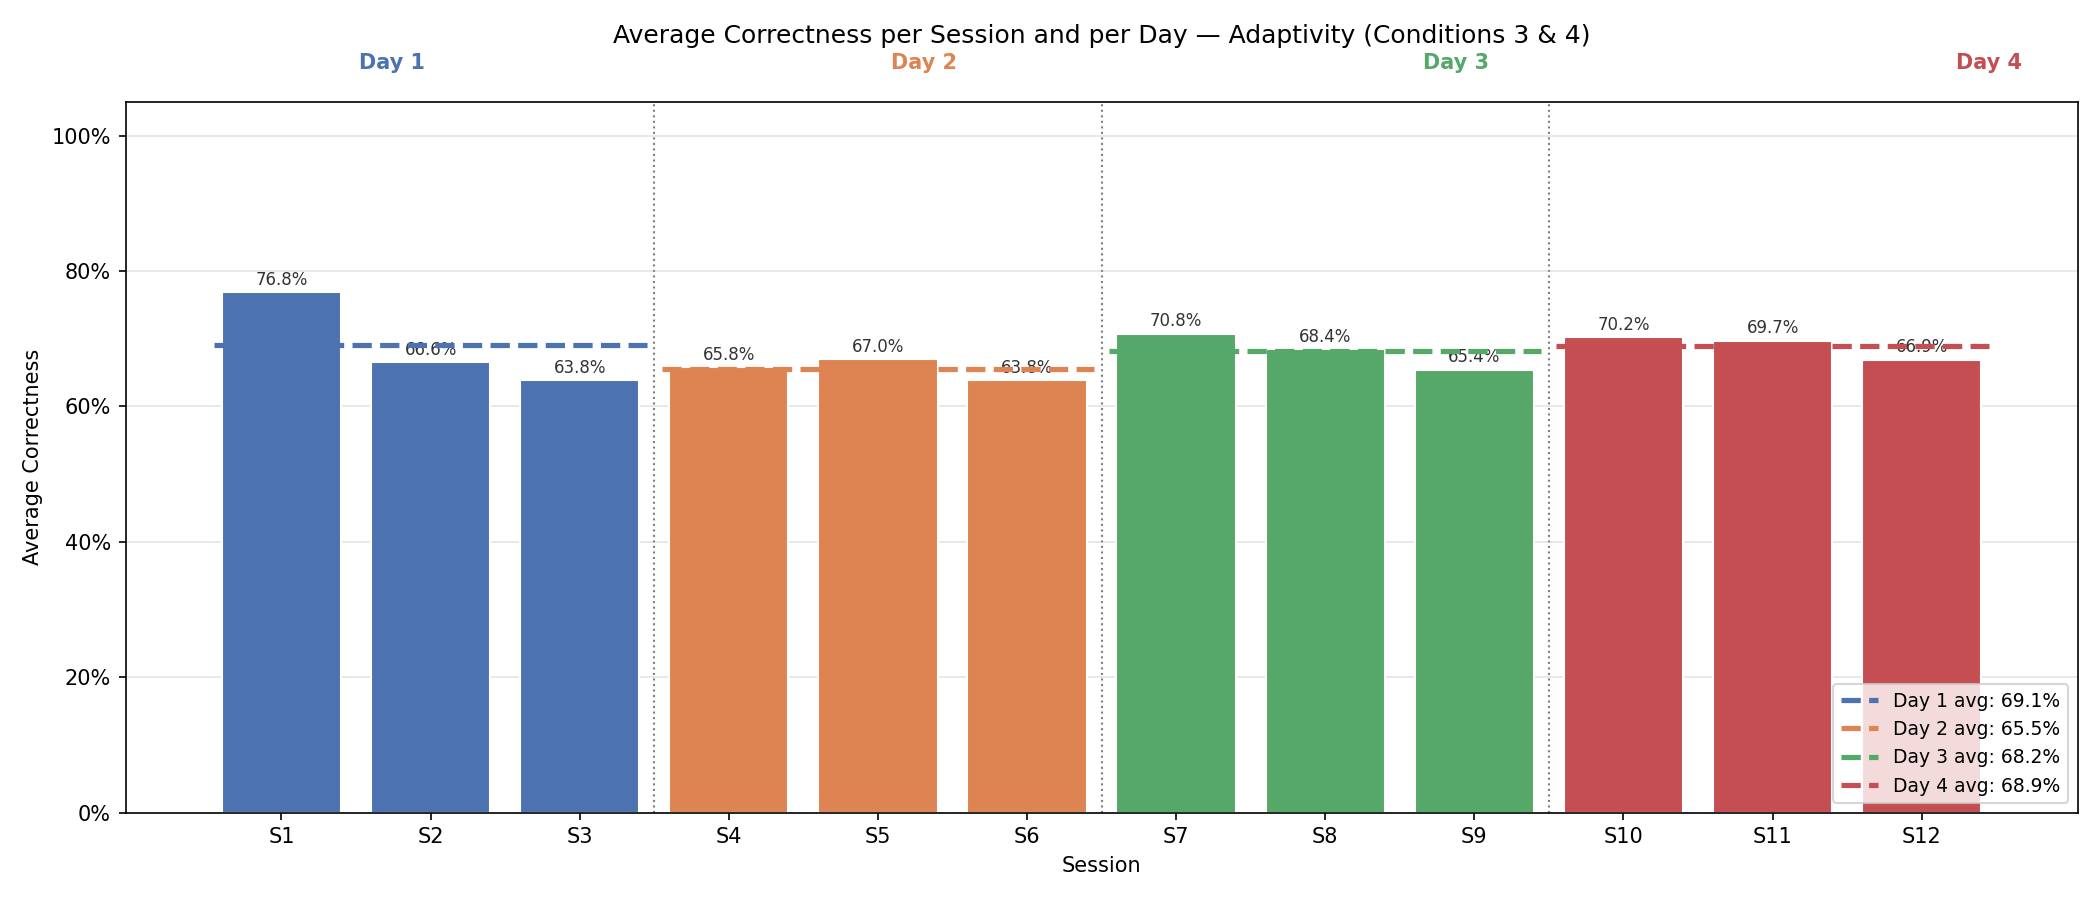
\includegraphics[width=\textwidth]{figures/correctness_by_session_adaptivity.png}
        \caption{Average correctness per block.}
        \label{fig:correctness-adaptivity}
    \end{subfigure}
 
    \vspace{0.4cm}
 
    \begin{subfigure}[t]{0.85\textwidth}
        \centering
        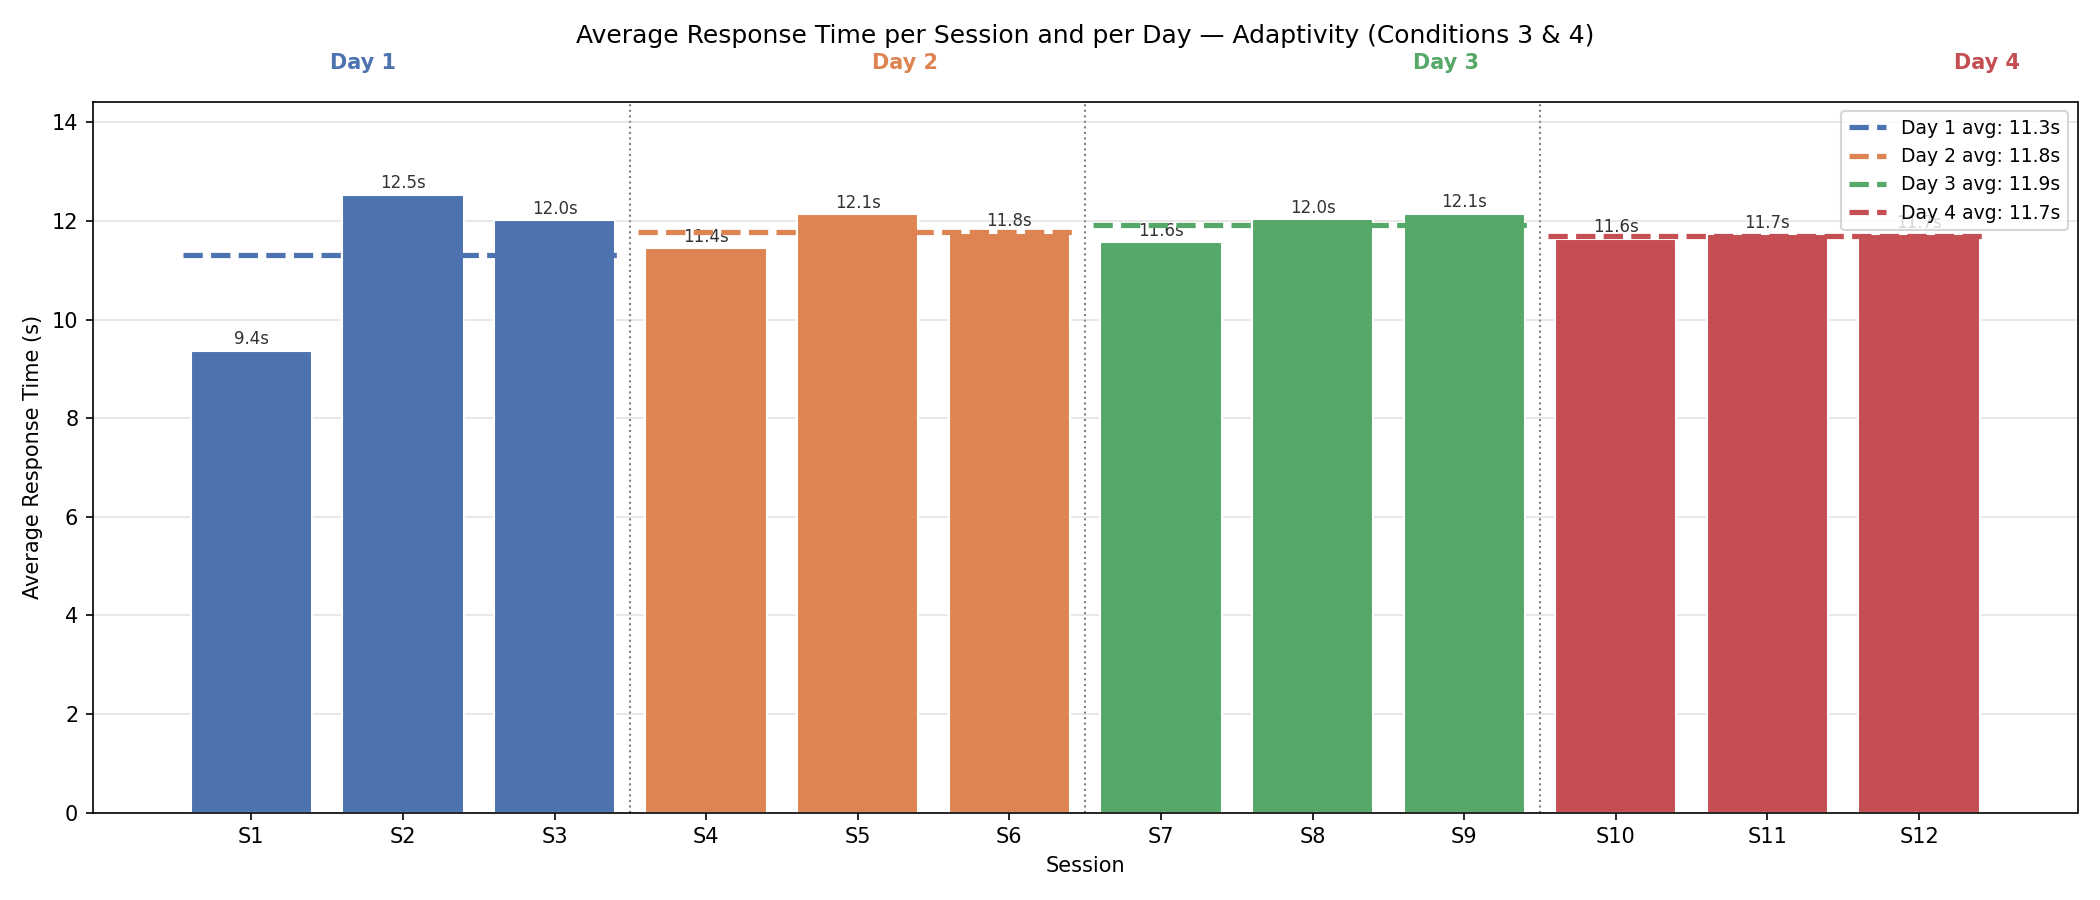
\includegraphics[width=\textwidth]{figures/response_time_by_session_adaptivity.png}
        \caption{Average response time per block.}
        \label{fig:rt-adaptivity}
    \end{subfigure}
    \caption{Average correctness and response time per block for the adaptive conditions (C and D), across the twelve blocks of the four training days.}
    \label{fig:within-day-adaptive}
\end{figure}
